% !Mode:: "TeX:UTF-8"
\chapter{box2D引擎的web移植}

\section{box2D简介}

Box2D是一个完全由C++实现的开源物理引擎\upcite{catto2011box2d},开源协议为zlib许可证。zlib许可是一个自由软件授权协议。Box2D开始的功能是用来模拟简单的二维刚体物理效果,比如加速度、阻尼、碰撞和破坏。后来Box2D引擎又加入了铰链、柔体、流体、粒子等效果。第一个版本是Erin Catto在2007年发布。

物理引擎不是计算机编程语言,也不是复杂繁琐的游戏引擎。但是游戏开发中广泛的使用物理引擎来实现各种物理效果,改善游戏的观赏效果,增强游戏的可玩性。

Box2D引擎已经内置了大量的物理算法,涵盖运动学、力学、空间几何的各种物理学数学知识。把复杂的物理模拟过程封装到程序“黑箱”之中,而把各种物理效果,以简单友好的API的形式暴露给开发者。开发者在开发时只需要简单的创建box2d中相应的对象并使用相应的函数,就可以模拟二维世界中的加速、阻尼、碰撞、破坏、引力斥力、柔体和流体效果。

\section{box2d的程序的特征}

和lua虚拟机以及SQLite数据库不同,我们需要得的不是一个“黑箱程序”。
而是一个需要把内部方法暴露出来,用来给别的语言调用的“白盒程序”,
或者叫框架或者类库。

这种需要时候,就需要使用webIDL技术。

本来,box2d是模块化开发的,可以在需要的时候,自主选取Common、Collision和Dynamics下的模块,按需引用。

但是,为了方便,需要把所以box2d相关的组件,一次性编译到一个JavaScript文件中,对外是一个闭包的形式\upcite{terrace2012javascript}。

\section{box2d程序的移植过程}

\subsection{box2d程序的移植过程}

box2d程序的移植过程如下所示:

\begin{enumerate}[itemindent=2em]
    \item 下载box2d源代码;
    \item 编写box2d的IDL文件,具体可见代码\ref{idl-box2d};
    \item 编写如下makefile;
\begin{verbatim}
LATEST =  Box2D_v2.3.1
STABLE =  Box2D_v2.2.1
PYTHON=$(ENV) python
VERSION := stable
BUILD := min

ifeq ($(BUILD), debug)
	OPTS = -O0 -g2
	LINK_OPTS = -g4 --llvm-lto 0 -s NO_FILESYSTEM=1 -s 
		NO_BROWSER=1 -s ASSERTIONS=2 --closure 0  -s DEMANGLE_SUPPORT=1 
else
	OPTS = -Os
	LINK_OPTS =  -O3 --llvm-lto 1 -s NO_FILESYSTEM=1 -s 
		NO_BROWSER=1  --closure 1  --js-transform "python bundle.py"
endif

ifeq ($(VERSION), latest)
	ACTIVE = $(LATEST)
	OBJECTS = \
	$(ACTIVE)/Box2D/Dynamics/Joints/b2MotorJoint.bc
else ifeq ($(VERSION), stable)
	ACTIVE = $(STABLE)
else
	ACTIVE = $(VERSION)
endif


OBJECTS += \
$(ACTIVE)/Box2D/Collision/b2BroadPhase.bc \
$(ACTIVE)/Box2D/Collision/b2CollideCircle.bc \
$(ACTIVE)/Box2D/Collision/b2CollideEdge.bc \
$(ACTIVE)/Box2D/Collision/b2CollidePolygon.bc \
$(ACTIVE)/Box2D/Collision/b2Collision.bc \
$(ACTIVE)/Box2D/Collision/b2Distance.bc \
$(ACTIVE)/Box2D/Collision/b2DynamicTree.bc \
$(ACTIVE)/Box2D/Collision/b2TimeOfImpact.bc \
$(ACTIVE)/Box2D/Collision/Shapes/b2ChainShape.bc \
$(ACTIVE)/Box2D/Collision/Shapes/b2CircleShape.bc \
$(ACTIVE)/Box2D/Collision/Shapes/b2EdgeShape.bc \
$(ACTIVE)/Box2D/Collision/Shapes/b2PolygonShape.bc \
$(ACTIVE)/Box2D/Common/b2BlockAllocator.bc \
$(ACTIVE)/Box2D/Common/b2Draw.bc \
$(ACTIVE)/Box2D/Common/b2Math.bc \
$(ACTIVE)/Box2D/Common/b2Settings.bc \
$(ACTIVE)/Box2D/Common/b2StackAllocator.bc \
$(ACTIVE)/Box2D/Common/b2Timer.bc \
$(ACTIVE)/Box2D/Dynamics/b2Body.bc \
$(ACTIVE)/Box2D/Dynamics/b2ContactManager.bc \
$(ACTIVE)/Box2D/Dynamics/b2Fixture.bc \
$(ACTIVE)/Box2D/Dynamics/b2Island.bc \
$(ACTIVE)/Box2D/Dynamics/b2World.bc \
$(ACTIVE)/Box2D/Dynamics/b2WorldCallbacks.bc \
$(ACTIVE)/Box2D/Dynamics/Contacts/b2ChainAndCircleContact.bc \
$(ACTIVE)/Box2D/Dynamics/Contacts/b2ChainAndPolygonContact.bc \
$(ACTIVE)/Box2D/Dynamics/Contacts/b2CircleContact.bc \
$(ACTIVE)/Box2D/Dynamics/Contacts/b2Contact.bc \
$(ACTIVE)/Box2D/Dynamics/Contacts/b2ContactSolver.bc \
$(ACTIVE)/Box2D/Dynamics/Contacts/b2EdgeAndCircleContact.bc \
$(ACTIVE)/Box2D/Dynamics/Contacts/b2EdgeAndPolygonContact.bc \
$(ACTIVE)/Box2D/Dynamics/Contacts/b2PolygonAndCircleContact.bc \
$(ACTIVE)/Box2D/Dynamics/Contacts/b2PolygonContact.bc \
$(ACTIVE)/Box2D/Dynamics/Joints/b2DistanceJoint.bc \
$(ACTIVE)/Box2D/Dynamics/Joints/b2FrictionJoint.bc \
$(ACTIVE)/Box2D/Dynamics/Joints/b2GearJoint.bc \
$(ACTIVE)/Box2D/Dynamics/Joints/b2Joint.bc \
$(ACTIVE)/Box2D/Dynamics/Joints/b2MouseJoint.bc \
$(ACTIVE)/Box2D/Dynamics/Joints/b2PrismaticJoint.bc \
$(ACTIVE)/Box2D/Dynamics/Joints/b2PulleyJoint.bc \
$(ACTIVE)/Box2D/Dynamics/Joints/b2RevoluteJoint.bc \
$(ACTIVE)/Box2D/Dynamics/Joints/b2RopeJoint.bc \
$(ACTIVE)/Box2D/Dynamics/Joints/b2WeldJoint.bc \
$(ACTIVE)/Box2D/Dynamics/Joints/b2WheelJoint.bc \
$(ACTIVE)/Box2D/Rope/b2Rope.bc


all: remove box2d.js
	@echo $(ACTIVE)"_"$(BUILD)".js is ready"

%.bc: %.cpp
	$(CXX) $(OPTS) -I$(ACTIVE) $< -o $@

box2d.bc: $(OBJECTS)
	$(CXX) $(OPTS) -I$(ACTIVE) -o $@ $(OBJECTS)

box2d_glue.cpp: $(ACTIVE).idl
	$(PYTHON) $(EMSCRIPTEN)/tools/webidl_binder.py $(ACTIVE).idl box2d_glue

box2d_glue.h: box2d_glue.cpp

box2d.js: box2d.bc box2d_glue.cpp box2d_glue.h
	$(CXX) $(LINK_OPTS) -I$(ACTIVE) -s EXPORT_BINDINGS=1 -s 
	RESERVED_FUNCTION_POINTERS=20 --post-js box2d_glue.js 
	--memory-init-file 0 -s NO_EXIT_RUNTIME=1 
	glue_stub.cpp $< -o build/$(ACTIVE)_$(BUILD).js

clean: remove
	rm -f $(OBJECTS)
	
remove:
	rm -f box2d.bc box2d_bindings.cpp box2d_bindings.bc box2d.clean.h box2d_glue.js box2d_glue.cpp WebIDLGrammar.pkl parser.out
\end{verbatim}    	
	\item 运行make LATEST 或 make STABLE 命令,得到box2d的js文件;
	\item 使用生成的js文件。
\end{enumerate}

在移植本软件时,同时下载了box2d 2.2.1 和 box2d 2.3.1 两个版本的源代码,
2.3.1版本新增了的功能主要是box2d引擎和GLFW结合相关的部分,
使用 make LATEST 可以得到 box2d 2.3.1 版本的js文件,
而 make STABLE 则是编译 box2d 2.2.1 版本的box2d源文件。

\subsection{box2d的程序的移植过程分析}

box2d的程序的移植过程分析如下:

\begin{enumerate}[itemindent=2em]
    \item 把c++文件编译成bc文件,即为llvm的字节码;
    \item 使用idl文件生成胶水文件;
    \item 把源代码和胶水文件(box2d\_glue.cpp,box2d\_glue.h,box2d\_glue.js )一起编译成js文件;
	\item 优化js文件。
\end{enumerate}

\subsection{box2d在浏览器中的运行效果}

图\ref{box2d-html}展示了box2d在浏览器中运行的效果。该Demo展示了box2d计算碰撞的结果,并把坐标传递到三维空间各个物体的x和y两个坐标值上。

\newpage

\begin{figure}[h!] % [h!] 表示尽量排在当前位置
    \centering
    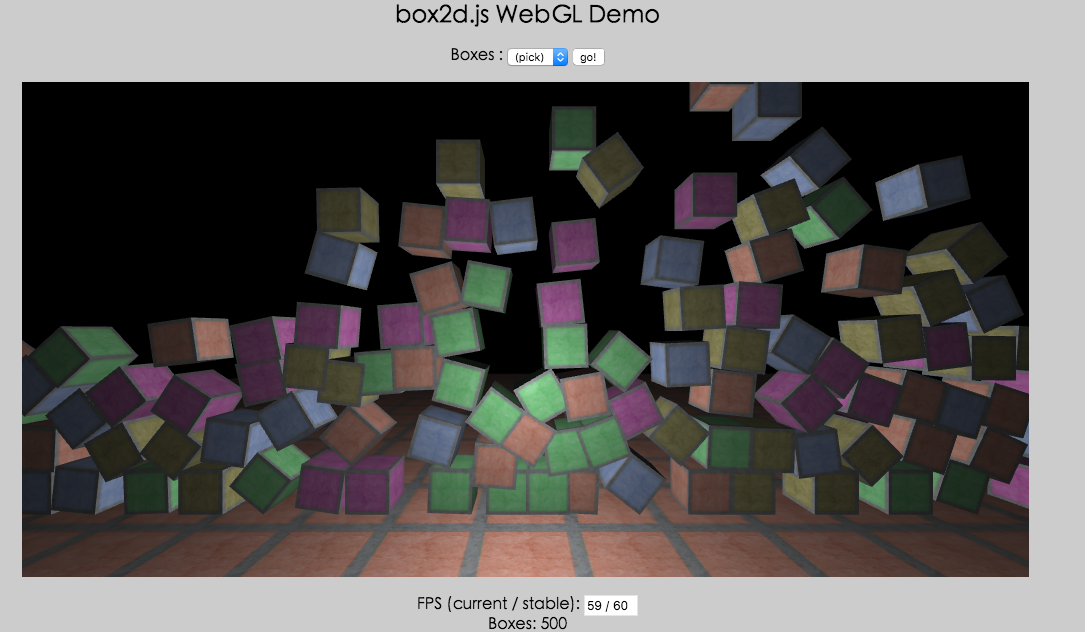
\includegraphics[width=450bp]{figure/pic/box2d-sample-html.png}
    \caption{box2d在浏览器中运行效果}
    \label{box2d-html}
\end{figure}

